\section{Study 5: remote emotion detection}
\label{s:study5}

\subsection{Introduction}

This study will describe my tests regarding the use of machine learning to detect the emotional state of subjects in my first experiment. The idea is to present this study as a planning for the second experiment. I will present the features used in the machine learning model, e.g. remote HR, eyebrow movement, etc, as a consequence of the previous studies.

The focus will be on the features used and the accuracy achieved. I imagine a plausiable hypothesis for this study is "is the model able to detect emotions with an accuracy that is better than chance?". In the discussion, I will present how some features influence the results, e.g. facial features only versus HR only. I will not mention the idea of user-tailored versus group-tailored, because it will make things too complex to describe and argue about. My idea is to save that discussion for upcoming papers.

\subsection{Analysis and methods}
  \subsubsection{Relevant feature extraction}
  Describe how the features are calculated and why they were selected (based on the info found in the literature and the results from previous studies).
  \subsubsection{Emotion classification}
  Describe how the model was trained, which includes how the calibration games were grouped, e.g. two for training, one for testing. Explain that neural networks were used because they are widely mentioned in the literature.
  \subsubsection{Evaluation of emotion classification}
  Describe how the machine learning model was tested and evaluated, e.g. mean accuracy of each subject, etc.
\subsection{Results}
\subsection{Discussion}
Discussion will be focused on the following: 1) was the machine learning model able to detect emotions with accuracy better than chance? 2) was the use of a multimodal approach (foundation of my thesis) better than the use of only facial features (or only HR)?.
\subsection{Conclusions}


%\section{Definition of inputs for the user-tailored model}
%\label{sec:closing-definition-inputs}

%The literature review presented in chapters \ref{ch:literature-physiological}, \ref{ch:literature-face} and \ref{ch:literature-multifactorial} indicates that a model based on several user signals, which is a multifactorial analysis, is more efficient for emotion detection. The mentioned chapters also highlight which of those signals can be remotely acquired within the context of this research via computer vision techniques.

%\begin{figure}[h]
%    \centering
%    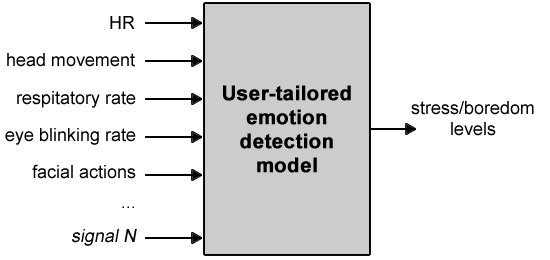
\includegraphics[width=0.6\textwidth]{figures/model-inputs-set.png}
%    \caption{Overall structure of the user-tailored emotion detection model regarding input (user signals) and output (stress/boredom levels).}
%    \label{fig:model-inputs-set}
%\end{figure}

%The user-tailored model proposed for this research might have $N$ input signals, varying from physiological ones, e.g. HR, to non-physiological ones, e.g. facial actions and head movements. Figure \ref{fig:model-inputs-set} illustrates the overall structure of the model. In order to be used in the model, an input signal needs to be supported by previous work regarding emotion detection, as well as be validated within the process of the proposed game-based calibration phase. Time and scope constraints limit the amount of input signals that can be implemented, evaluated and used in this research. As a consequence, a study will be conducted to investigate, validate and initially implement two of those signals into the proposed model: HR and facial activity (which includes head movement, lips activity, etc).

%The techniques and works presented in chapter \ref{ch:literature-face}, which relate to face detection and emotion estimation, suggest that facial analysis is an important component of a multifactorial emotion detection model. Empirical analysis of the data from the first experiment also suggest that individualities regarding facial activities do exist and could be used to estimate emotional states on a user-tailored basis \parencite{bevilacqua2016variations}. As described in section \ref{ch:literature-face-emotion-detection}, facial actions, head movement, lips/eye/mouth activity and distance measurements of detected facial landmarks are viable and proven sources of information for emotion detection.

%Regarding physiological signals, results indicate that the average HR mean for players during the last minute of gameplay is greater than the average HR mean during the second minute of gameplay (chapter \ref{ch:experiment1}, section \ref{s:study3}). The findings are aligned with and reinforce previous research that indicates higher HR mean during stressful situations in a gaming context. The findings also suggest that changes in the HR during gaming sessions is a promising indicator of stress.

%The study will involve the definition of how those two signals will be used as inputs for the model. Facial actions, for instance, will probably be detected and measured by the euclidian distance of the facial landmarks. A vector containing the distances will be evaluated as the input for the model. Regarding the HR, its mean and standard deviation during a particular analysis window will be evaluated as input for the model. A software for the detection of those two signals will be created and used to analyse the video recordings of the first experiment (chapter \ref{ch:experiment1}). The inclusion or exclusion of a component of a signal, e.g. variations of the distances of the lips landmark points, will be based on the accuracy to detect them and the frequency they appear in boring and stressful part of the calibration games.

%\section{Investigation of machine learning techniques}
%\label{closing:investigation-machine-learning}

%The majority of the previous work found in the literature mention the use of machine learning techniques to model user signals into emotional states. Different models and accuracy results are mentioned, which depend on several particularities of the approach used by the authors. A machine learning model will also be used by this research as a user-tailored emotion detection model.

%\begin{figure}[h]
%    \centering
%    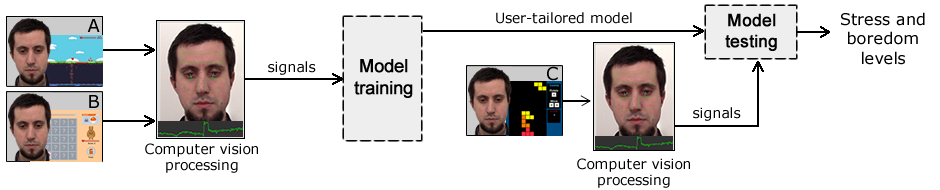
\includegraphics[width=\textwidth]{figures/machine-learning-investigation.png}
%    \caption{Iteration of a 3 fold cross validation performed on the video of a gaming sessions with 3 games, i.e. A, B and C. The videos of two calibration games, e.g. A and B, are used to train the machine learning model, while the video of the third calibration game, e.g. C, is used to test the model.}
%    \label{fig:machine-learning-investigation}
%\end{figure}

%A systematic study and accuracy evaluation will be performed to select the proper machine learning technique to be used in the model. The evaluation process will be conducted on each one of the selected (and competing) machine learning techniques using the video recordings of experiment 1. The evaluation is based on a 3 fold cross validation process, illustrated in Figure \ref{fig:machine-learning-investigation}. Initially the input signals for the emotion detection model (defined in the previous task, section \ref{sec:closing-definition-inputs}) will be extracted from two, e.g. A and B, of the three games played by a user and used to train the emotion detection model. The thrid game, e.g. C, that was left out of the training will be used as a testing set: user signals will be extracted from the video of that game and fed into the trained emotion detection model, which will output the predicted emotional state of the user. The 3 fold cross validation process is repeated three times, each one of them leaving out of the training phase a different game, i.e. A and B are used for training and C is used for testing, A and C are used for training and B for testing, and finally B and C are used for training and A for testing.

%\begin{figure}[h]
%    \centering
%    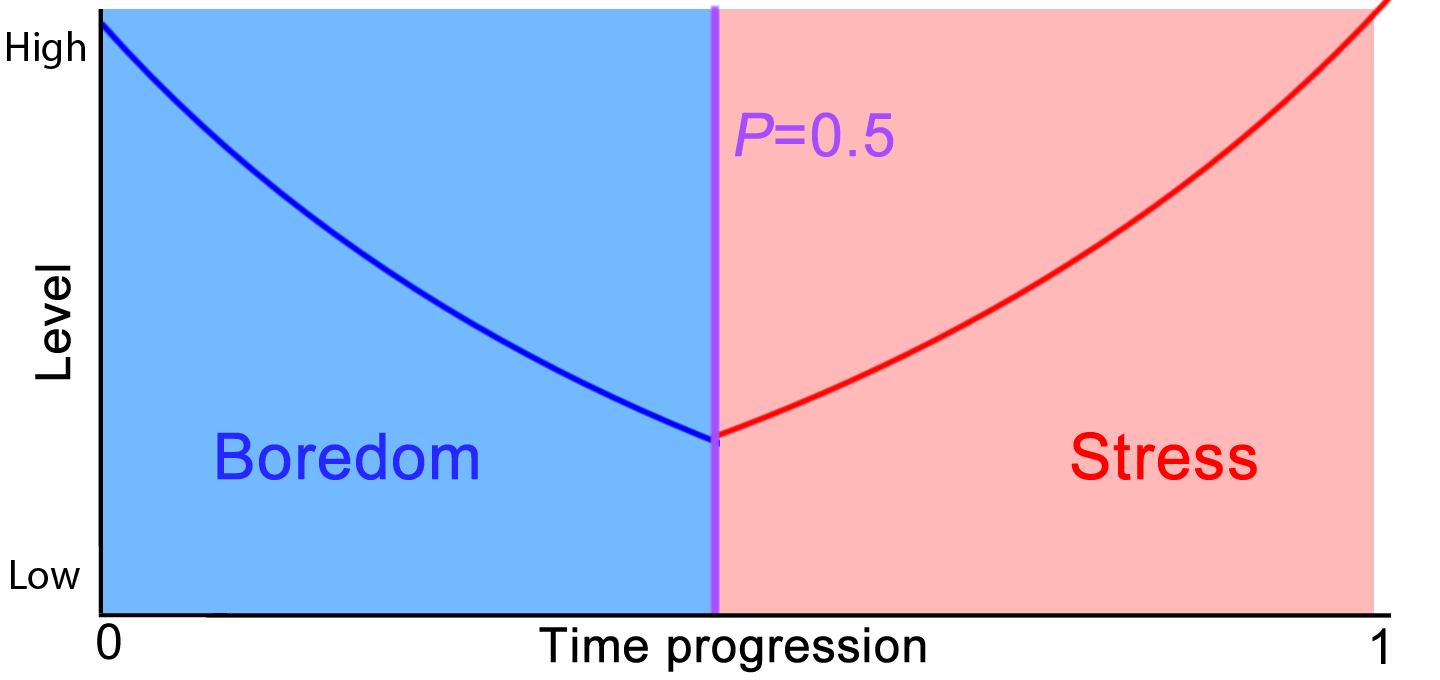
\includegraphics[width=0.8\textwidth]{figures/machine-learning-labeling-approach-A.png}
%    \caption{Labeling approach for the training of the user-tailored model based on a fixed point of division $P$ for both boredom and stress samples.}
%    \label{fig:machine-learning-labeling-approach-A}
%\end{figure}

%The video recordings that will be used in the tasks are related to experiment 1, whose games were designed to work as calibration games. As previously described in section \ref{sec:contributions}, those calibration games feature a progression from a boring to a stressful state. That configuration will be used as the foundation for the labeling process of emotional states during the training of the model, as well as ground truth for its testing.

%\begin{figure}[h]
%    \centering
%    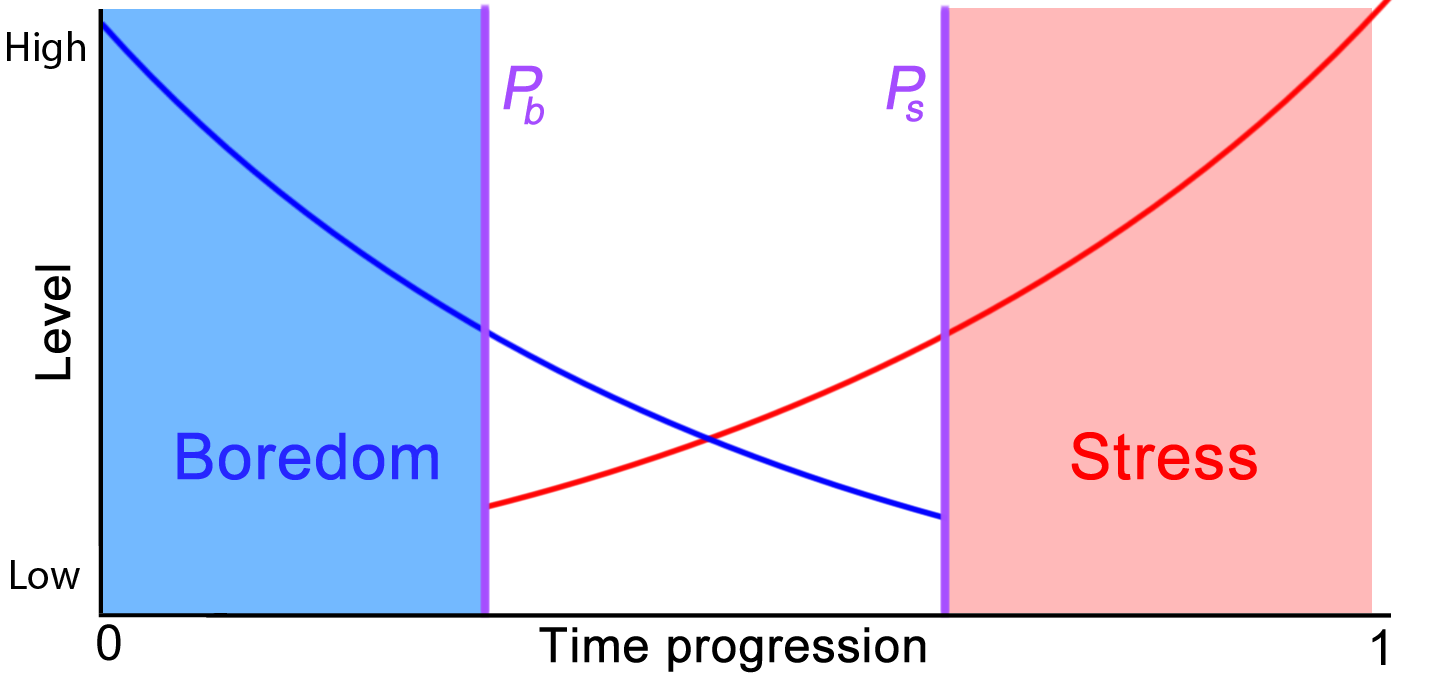
\includegraphics[width=0.8\textwidth]{figures/machine-learning-labeling-approach-B.png}
%    \caption{Labeling approach for the training of the user-tailored model based on varying points of division: $P_b$ (boredom samples) and $P_s$ (stress samples).}
%    \label{fig:machine-learning-labeling-approach-B}
%\end{figure}

%The training of the emotion detection model will be conducted according to two different strategies. In both approaches, the two games used as training sets will have their user signals sampled at a fixed interval of $T$ seconds, being $T$ empirically defined. The labeling of a sample as boredom or stress, however, will be different.

%Approach \textbf{A}, illustrated in Figure \ref{fig:machine-learning-labeling-approach-A}, assumes that $P$ represents the time progression of each game, e.g. $P=0$ is the starting point of the game and $P=1$ is its end point. Each game will then be divided in two equal parts ($P=0.5$). Samples from the first half of the game will be labeled as boredom, while samples from the second half will be labeled as stress. The division is based on the assumption that the middle of the games accurately separates in time the self-reported perceptions of boredom and stress made by the subjects.

%Approach \textbf{B}, illustrated in Figure \ref{fig:machine-learning-labeling-approach-B}, has each game divided in two parts: boredom, i.e. $P_b$, and stress, i.e. $P_s$, whose size (duration in time) will be calculated based on the self-reported answers given by subjects regarding boredom and stress. Samples from the $P_s$ part will be labeled as stress, while the samples from the $P_b$ part will be labeled as boredom. Approach \textbf{B} tries to mitigate the assumption that the middle point of the games perfectly divides the perceptions of boredom and stress. The approach accounts for the informed levels of boredom and stress of the subject, labeling only the samples within the areas more likely to accurately reflect the self-reported emotional states.

%The testing process will be similar for both approaches \textbf{A} and \textbf{B}. Samples from the game used as a testing set will be collected at a fixed interval of $K$ seconds, which will be larger than $T$ and also defined empirically. The associated labeling of the samples will be based on their position according to the rules of division points, i.e. $P$, $P_b$ or $P_s$. Sample points that eventually are not labeled, e.g. middle points in approach \textbf{B}, will be labeled as neutral.

%Following the described procedure, after all machine learning techniques are tested, they will have several resulting accuracy scores. The technique with the highest mean for the accuracy score will be selected. The following machine learning and classification techniques will be initially used in the tests: Support Vector Machine (SVM) using a radial basis, C-Support Vector Classification (C-SVC) using a linear kernel, K-nearest neighbours (K-nn), AdaBoost using nearest mean classifiers, Naive Bayers, and neural networks probably represented by convolution networks (convnets). Previous work \parencite{samara2016sensing,akakin2010spatiotemporal} also suggest a process involving decision fusion or a hierarchy of two or more classifiers working on different feature sets to improve prediction rates. Those approaches will probably be investigated as well.

%\subsection{Challenges and unresolved issues}

%One of the main unresolved issues regarding the use of a machine learning model is regarding its input features. Computer vision will be used to remotely extract a set of signals from the users, e.g. HR and the position of facial landmarks, however how those signals will be packeged as inputs for the machine learning model is still undefined.

%The current idea is to use a direct and discrete approach where the set of extracted signals from each frame of the video being analyzed is used as is. This approach does not explicitly feed the model with information regarding the variations of the extracted signals, e.g. HR decreased 5 bpm in the last 10 seconds, instead current information from each frame is used as input, e.g. HR is 60 bpm now. The approach relies on the principle that the machine learning model will recognize any patterns regarding the variation of signals among the different samples over time, modeling those patterns as the desired mapping of emotional states.

%Another possible solution is to provide the model with the variations of the signals, which demands a pre-processing of the extracted signals before feeding them into the model. In such scenario, each extracted signal will be accompanied by additional data, e.g. standard deviation, mean, etc. Ideally the machine learning model will better account for the variations of the signals and the emotional states. If a convolutional neural network is used as a machine learning solution, for instance, each signal can be used as input to the model in the form of a matrix. In that case each row of the matrix contains a segment of the signal at different times and the convnet will automatically find a way to model such changes into emotional states.
